\begin{refsection}
    \renewcommand{\thefigure}{\arabic{figure}}

    \chapterTwoLines
    {Mapas da cidade}
    {textos, imagens e imaginários}
    \label{chap:mapadacidade}
    
    \articleAuthor{Leonardo da Silva Claudiano}
    {Doutorando em História Social pela Pontifícia Universidade Católica de São
    Paulo (PUC-SP), com bolsa CAPES. Pesquisador do Núcleo de Estudos de
    História Social da Cidade (NEHSC/PUC-SP). Membro do Grupo de Estudos
    Literatura e Ditaduras (GELD/PUC-SP); e membro do Grupo de Estudos em
    História e Literatura da Pontifícia Universidade Católica de Minas Gerais
    (GEHISLIT/PUC-Minas). Lattes ID: 0306.6809.5977.0318. ORCID:
    0000-0003-2010-3501. E-mail: leonardo.claudiano@gmail.com.}

    \begin{galoResumo}
        \marginpar{
            \begin{flushleft}
                \tiny \sffamily
                Como referenciar?\\\fullcite{SelfClaudiano2021}\mybibexclude{SelfClaudiano2021},
                p. \pageref{chap:mapadacidade}--\pageref{chap:mapadacidadeend},
                \journalPubDate{}
            \end{flushleft}
        } O presente artigo tem como objetivo buscar as representações da
        cidade de São Paulo das duas primeiras décadas do século XX, por meio
        do diálogo entre imagens e textos produzidos no período, com destaque a
        António de Alcântara Machado. Pela articulação entre a concretude
        citadina e algumas produções fotográficas e literárias, pretendemos
        analisar a formação de determinados imaginários urbanos ligados à
        modernidade. Igualmente, intentamos contribuir ao debate entre História
        e Cidade.
    \end{galoResumo}
    
    \galoPalavrasChave{História e Cidade. História e Literatura. Modernidade.}
    
    \begin{otherlanguage}{english}
    
    \fakeChapterTwoLines
    {City maps}
    {texts, images and imaginary}

    \begin{galoResumo}[Abstract]
        This article aims to seek representations of the city of São Paulo in
        the first two decades of the twentieth century through a dialogue
        between images and texts produced in that period, with emphasis on
        António de Alcântara Machado. Through the articulation between city
        concreteness, and a few photographic and literary productions, we intend
        to analyze the formation of some urban imaginary linked to
        modernity. Likewise, we wish to contribute to the debate between
        History and City.
    \end{galoResumo}
    
    \galoPalavrasChave[Keywords]{History and City. History and Literature. Modernity.}
    \end{otherlanguage}

    \section{Introdução}

    Ao nos debruçarmos sobre as plantas da cidade de São Paulo\footnote{Disponível em \url{http://smul.prefeitura.sp.gov.br/historico_demografico/1920.php}. Acesso em 12 abr. 2021.}, dos anos vinte, encontramos com facilidade a Rua Oriente. Localizada nos arredores do ``BRAZ'' e ``Pary'', ela se apresenta como um corte diagonal, em meio aos quarteirões que se desdobram por todos os lados. No mapa, o adensamento populacional, de certa forma, guarda relação com as diversas letras e linhas que representam aquele bairro operário. A caligrafia cuidadosa, na folha amarelada, nomeia vias que, por vezes, sobrepõem-se umas às outras e formam um amontoado que não se distingue: a cartografia urbana é, aos nossos olhos, caótica na sua apreensão em escala. Sentimos a densidade da região central e seus bairros circundantes. Da mesma forma, ao nos afastarmos e procurarmos o olhar em perspectiva, temos longos espaços vagos, alguns novos loteamentos e outros núcleos a ocupar as bordas --- ``Villa Gomes Cardim'', à leste; ``Villa Leopoldina'', à oeste.  

    O mapa é fundamental para compreendermos a cidade e seu crescimento. Sozinho, entretanto, torna estático um processo altamente dinâmico. É preciso o contraponto com plantas passadas e futuras, para que, em partes, o movimento se revele: ao norte, em 1916\footnote{Planta da Cidade de São Paulo, 1916 --- Imagem: Anexo \ref{annex:sp1916}.}, ``SANT'ANNA'' tem como companhia a Cadeia Pública e parcas linhas de ligação ao Centro; já em 1924\footnote{Planta da Cidade de São Paulo, 1924 --- Imagem: Anexo \ref{annex:sp1924}.}, a ``Villa Guilherme'' se avizinha e a ``Villa Maria'' tem suas quadras a apontar ocupações futuras.  

    A análise pode, então, aprofundar-se. Para melhor entendermos as motivações desta expansão, articulamos à cartografia outras fontes, como relatórios técnicos, imagens, textos produzidos por literatos, historiadores, et cetera. Sevcenko, em sua importante e referencial obra ``Orfeu Extático na Metrópole'' \citeyear{Sevcenko2014Orfeu}, constrói a argumentação assentada em cronistas da imprensa paulistana. Ao colocá-los em diálogo com outros documentos e linguagens, extrai recortes interessantes da cidade: imagens dos frenéticos anos vinte, resultado de uma morfologia urbana aparentemente indefinida, entrecortada de temporalidades e estilos arquitetônicos diversos, pontuada por cortiços e habitações operárias; vias dotadas de iluminação elétrica, modernos bondes e ruas descalçadas. Nesse ambiente concreto, vivências e sociabilidades se desenrolam a afirmar, negar e ressignificar os próprios traçados pré-definidos. Tais imagens urbanas foram compartilhadas pelos habitantes e, algumas, perpetuadas no tempo. A nós, chegam ecos abafados, camuflados, também do que se pretendeu emudecer. Narrativas que deliberadamente foram esquecidas, mas que deixaram rastros, vestígios na cidade em palimpsesto.  

    A expansão urbana, a qual nos referimos, silenciou a segregação que promoveu, ao reforçar, única e discursivamente, o progresso e a modernidade que fizeram da localidade esquecida no planalto a maior metrópole da América Latina. Nicolau Sevcenko nos lembra que, por detrás do redesenho citadino, do crescimento vertiginoso de São Paulo, encontrava-se o ``mais danoso agente especulador, que comprometeu definitivamente o futuro da cidade, forçando seu desenvolvimento em bolsões desconexos'' \cite[p.~122]{Sevcenko2014Orfeu} --- a empresa de capital canadense-anglo-americano, Light and Power: 

    \begin{quotation}
        A Light, naturalmente, era a peça decisiva no modo de expansão da cidade. Localizando as paradas finais de suas linhas em pontos extremos e de população rarefeita --- Penha, Lapa, Santana, Ipiranga, Vila Mariana, Pinheiros ---, ela gerou fluxos irradiados de valorização imobiliária que, seguindo as direções de seus trilhos, suscitavam a criação de loteamentos em áreas remotas. Essas áreas, ao obterem os serviços básicos de transporte, eletrificação e gás, fornecidos pela própria Light, geravam zonas intermediárias entre esses locais já dotados de infra-estrutura e o centro da cidade, tornadas automaticamente supervalorizadas, o que elevava os preços dos terrenos e aluguéis em níveis exponenciais. \cite[p.~123--124]{Sevcenko2014Orfeu}
    \end{quotation}

    Assim, os vazios que circundam a área central da cidade, nas plantas que nos servem de base, ganham novos significados. A imensidão, apenas perturbada por linhas de conexão a quarteirões distantes, é preenchida, por nossa análise, com a historiografia. E o olhar, apura-se. Por exemplo: ao buscarmos a ``LAPA'', na planta de 1916, localizamos, nas margens extremas do oeste, o arrabalde distante. Para além, nada mais compõe o traçado urbano. Aquém, ausências só interrompidas nos limites do ``Parque Antarctica''. Seguindo ao Centro, ``Villa Pompeia'' é mero esboço; ``Perdizes'', poucos traços.  É nas imediações da ``SANTA EPHIGENIA'' que o nanquim se carrega ao representar ruas e quarteirões. A partir da cartografia de 1924, o adensamento é evidente. A mancha central se amplia, avança em novas vias. As linhas isoladas de ``Perdizes'' se unem aos traços da ``STA. CECILIA''. A ``Villa Pompeia'' é firmada em quadrantes extensos. A ``LAPA'' deixa de ser a borda do mapa: à esquerda, o ``Alto da Lapa'' é seu prolongamento, e a ``Villa Leopoldina'' toca os limites do Rio Pinheiros; depois, o caminho para Sorocaba.  

    Vale ressaltar que fatos semelhantes se observaram por toda a cidade, planejada e executada, principalmente, pelo capital especulativo, personificado na figura da Light. Evidente que o processo não se fez de forma sinérgica, harmônica. Da mesma forma, nem toda intervenção se resumiu aos interesses financeiros mais imediatos. A urbanização é fenômeno conflituoso, com discussões que percorrem inúmeras instâncias. Por ora, queremos chamar atenção aos embates que se fizeram pelo corpo social, entre aqueles que pensaram e edificaram um modelo de cidade, e os que a viveram cotidianamente. Pela disparidade das forças, as confrontações revelaram-se sinuosas, e a cidade imposta foi aceita para ser subvertida. Subversão que se fez --- e se faz --- com base na concretude e circunstâncias determinadas. Em outras palavras: todo traçado urbano contém em si tanto os mecanismos do poder político e econômico, quanto a insubordinação que o redesenha, com sentidos e usos que escapam ao que foi inicialmente pensado. A ``LAPA'' periférica, afastada, era, para a Light, \textit{locus} especulativo; para seus habitantes, pertencimento, identidade, memória. Temos, assim, que: 

    \begin{quotation}
        A modificação do espaço de uma cidade, dando a ela forma e feição, contêm em si um projeto político de gerenciamento do urbano em sua totalidade. É, por um lado, uma tarefa de profissionais especificamente habilitados para tal --- urbanistas, arquitetos, engenheiros ---, mas também comporta o que se poderia chamar de intervenção do cotidiano. Ou seja, esse espaço sonhado, desejado, batalhado e/ou imposto é, por sua vez, também reformulado, vivido e descaracterizado pelos habitantes da urbe, que, a seu turno, o requalificam e lhe conferem novos sentidos. \cite[p.~16]{Pesavento2002Imaginario} 
    \end{quotation}

    Interessa-nos, aqui, abordar a relação dialética entre as cidades pensadas, realizadas, e a urbe vivenciada, sentida, ressignificada. A Rua Oriente, com a qual abrimos este artigo, vale-nos não apenas pela sua localização na planta de São Paulo. Tampouco a queremos, se pautada apenas pelo Requerimento n. 78, da Sessão Ordinária da Câmara, de 17 de abril de 1920:

    \begin{quotation}
        Dado o estado em que se acha o calçamento a macadam da rua Oriente, impossibilitando por completo o transito que não é pequeno por aquella rua, solicito da Prefeitura a fineza de uma providencia no sentido de ser, com a maxima urgencia, substituido aquelle systema de calçamento pelo de parallelepipedos de pedra. Pela rua do Oriente, é hoje feito, em maior escala, o transporte de cargas para os armazens do Pary e grande numero de fabricas ali existentes. --- Sala das sessões, 17 de abril de 1920 --- \textit{M. Pereira Netto.} --- A' Prefeitura.\footnote{Sessão Ordinária da Câmara, de 17 de abril de 1920 (S.O. 13 de 1920), Requerimento n. 78 de 1920. Disponível em \url{https://www.saopaulo.sp.leg.br/static/atas_anais_cmsp/anadig/Sessoes/Ordinarias/013SO1920.pdf}. Acesso em 15 abr. 2021.}
    \end{quotation}

    Vale-nos porque foi na Rua Oriente que Gaetaninho viveu e teve sua vida abreviada pelo bonde, na cidade onde o lúdico e o fluxo colidiram de morte. Como nota-se, dentre os muitos discursos, é pelo literário que percorreremos os quarteirões de São Paulo. As plantas da cidade ganharão vida --- e crime --- por meio de Gaetaninho, principal personagem criado por António de Alcântara Machado, em ``Brás, Bexiga e Barra Funda'' (1927). Ao longo do artigo, buscaremos, também, o diálogo com outras fontes e linguagens, para assim estabelecermos alguns possíveis caminhos na procura pelas imagens da cidade que emergem de textos, fotografias, cinema. O espaço vai de Nova York a São Paulo. Apesar de contextos diferentes, nossa ideia é demonstrar as representações que partem do concreto e a ele retornam, dos imaginários que surgem das pedras e a elas ressignificam.

    \section{Cidades e representações}

    São inúmeros os estudos que se dedicam às cidades. A diversidade de abordagens acompanha a multiplicidade de produções e, praticamente, todos os campos das ciências ou das artes, dela se ocuparam --- e ocupam. Pelos olhares da História, as possibilidades de entradas são igualmente amplas e, segundo questões postas pela contemporaneidade da investigação, certas características epistemológicas se firmam, em maior ou menor grau. Não é o nosso objetivo, aqui, traçar a elaboração deste campo temático ou o seu percurso historiográfico. Entretanto, algumas abordagens merecem destaque, principalmente porque revelam, para além das análises que empenham, questões, anseios e intenções de seu tempo. Partimos, assim, da História da Cidade que se realiza sem preocupações teóricas consistentes. Pautada pelo encadeamento de fatos --- espécie de biografia, amparada em uma série de dados, nomes, e demais informações que não se articulam, apenas procuram reforçar a grandeza a ser decantada, o futuro promissor a se realizar, uma vez que os indícios já se mostravam em pretérito; damos destaque, ainda, às investigações que a veem como ``\textit{locus} da acumulação de capital, como o epicentro da transformação capitalista do mundo'' \cite[p.~77]{Pesavento2014Historia}. Palco da luta de classes, o espaço urbano reproduz a lógica e as contradições da produção econômica. Por fim, a vertente da História Cultural, pela qual nos pautaremos:  o olhar que encara a urbe por meio de uma relação que, com base no concreto, ultrapassa-o. Além da materialidade, adiante das pedras que a formam, a procura pela significação de seus traçados na elaboração de imagens, discursos: a cidade como representação. Dito de outra forma, aos dados técnicos, ao campo de embates, interessa-nos as linguagens e as vivências que os percorrem, em afirmações e/ou ressignificações --- a gênese de um imaginário urbano, sempre mutável, e igualmente palco de lutas.  

    Marshall Berman, em ``Um século em Nova York: espetáculos em Times Square'' \citeyear{Berman2009Seculo}, parte das representações sobre a Times: cartões postais, filmes, musicais, fotografias, anúncios publicitários, et cetera --- e delas, dialeticamente, pelos espaços e imaginários, refaz o percurso centenário, entrecortado de sentidos.  

    \begin{quotation}
        Quero com este livro mergulhar na cultura de congestão da Square: congestão não só de pessoas, edifícios, carros, letreiros, mas, o que é o mais fascinante de tudo, congestão de significado. É um lugar em que podemos nos afogar ou lutar para nos manter à tona numa superabundância de significados. \cite[p.~16]{Berman2009Seculo} 
    \end{quotation}

    \begin{figure}[ht]%
        \centering%
        \caption{Cartão-postal ``Garota do Times'', 1903 (Museum of the City of New York)}%
        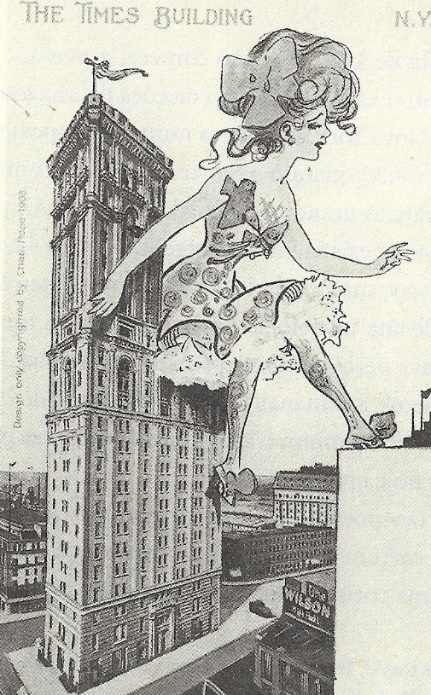
\includegraphics[width=.35\textwidth]{articles/15-cidade-em-mapas-text/cartao-postal-nyc.jpeg}%
        \caption*{Fonte: \textcite[p.~12]{Berman2009Seculo}. Autor desconhecido.}%
        \label{fig:cartao-postal-nyc}%
    \end{figure}%

    Sua perspectiva de análise é fruto dessa aproximação entre a materialidade espacial, vivências humanas e os significados imanentes e transcendentes dessas relações. A fotomontagem (figura \ref{fig:cartao-postal-nyc}), de 1903, na qual a Times Tower, em toda sua imponência de vidros e aços, serve de apoio ao cartum de uma garota, é fundamental para compreendermos o trajeto que Berman nos propõe: sentada, ombros e pernas à mostra, cabelos despenteados a emoldurar o rosto que se compõe com sorrisos, ela se mostra totalmente à vontade no espaço público que a acolhe. Ao longo dos anos, este local se afirmará receptivo, como no período do pós-guerra. Berman lembra-nos do filme ``Um dia em Nova York'' \citeyear{KellyAndDonen1949Dia}, com os marinheiros a saírem pelas ruas de uma cidade que amanhece deslumbrante, convidativa. Acompanhados da canção ``New York, New York'', as câmeras os seguem por ruas e avenidas solares --- um corte que ``dura menos de cinco minutos, mas contém imagens luminosas que misturam os marinheiros com muitos dos locais mais espetaculares da cidade'' \cite[p.~141]{Berman2009Seculo}. Pelos quarteirões nova iorquinos, eles vivem, apaixonam-se. Nós, espectadores, sentimo-nos parte. Temos a cidade em oferenda, aberta, atraente em possibilidades. Entretanto, algo muda à medida que avançamos pelas décadas, e as produções sobre a Times acompanham estas transformações. Nos anos setenta, o boulevard torna-se sujo. O colapso material e econômico gera uma espécie de decadência ``espiritual''. As representações da Square se fazem imundas, sombrias: o neon dos anúncios não ilumina, antes parece reforçar a escuridão que o envolve. O clima é \textit{noir}, torpe, de becos fétidos e lixos pelas ruas. Apreensivos, ficamos em suspenso. Marshall Berman se debruça sobre ``Taxi Driver'' \citeyear{Scorsese1976Taxi} e, no táxi de Travis (Robert de Niro), somos conduzidos por lugares detestáveis.  Esta, certamente, não é a Nova York na qual uma garota se sentaria descompromissada na Times Tower. 

    Notamos, nestes exemplos, a relação íntima e conflituosa que existe entre as fontes concretas e palpáveis da urbe, e as representações que dela proveem, em contextos distintos.

    \section{Imagens e textos urbanos}

    Uma vez que ``as cidades são antes de tudo uma experiência visual'' \cite[p.~237]{Bresciani2014Historia}, insistiremos um pouco mais nas representações imagéticas, agora em abordagens fotográficas. Vale dizer que a morfologia urbana e seus traçados, captadas pelas lentes, compõem a iconografia da imagem, que é literal e descritiva \cite{Kossoy2014Fotografia}. Ou seja, os elementos da cena, num primeiro momento, dizem o que está expresso. A partir daí, por outros cruzamentos documentais, extraímos o mais importe: as intenções, representações. Buscamos a imagem além da imagem.  

    Curioso notar que algumas delas, ficam. Principalmente as que enfocam paisagens urbanas. De certa forma, tocamos num paradoxo: diante do apelo imagético intenso e constante, nossas retinas vagam de uma à outra, porém se retardam em poucas e, dentro desse número diminuto, uma quantidade ainda menor permanece indelével, sem a necessidade de novo contato para reavivá-las totalmente. As imagens que se sustentam em nós, são as que dialogam com algo que possuímos previamente, numa espécie de intercâmbio entre o que vemos e o olhar que trazemos. Determinados instantes se perpetuam, no plano individual ou coletivo, pelo discurso que nos constitui em aproximação com o dizer da imagem. 

    ``O que a Fotografia reproduz ao infinito só ocorreu uma vez: ele repete mecanicamente o que nunca mais poderá repetir-se existencialmente'' \cite[p.~14]{Barthes2015Camera}. O beijo entre o marinheiro George Mendonsa e a enfermeira Greta Zimmer Friedman, em 14 de agosto de 1945, na Times Square, talvez seja a foto mais emblemática da Segunda Guerra fora de um campo de batalha (figura \ref{fig:enfermeira-marinheiro}). Berman dedica um capítulo especial para analisá-la, no já citado estudo ``Um século em Nova York: espetáculos em Times Square'' (2009). Por meio da fotografia, parte às reflexões estéticas que contribuíram para sua perpetuação nos imaginários e, somadas à percepção de ``Boa Guerra'', travada para proteger a América e o mundo contra o mal real e poderoso'' \cite[p.~92]{Berman2009Seculo}, encontra, aí, os componentes fundamentais na preservação do casal cujo beijo não termina. Mas Berman nos chama a atenção, igualmente, para o cenário onde a ação se desenrola: Times Square. Para ele, um microcosmo da cidade moderna, de possibilidades e fracassos, de reconhecimento e anonimato. Palco onde um gesto de afeto decorre e traz nos seus referentes a guerra que deixou pelo caminho milhões de mortos. Na foto, ambos uniformizados, cada um trazendo em si as vestimentas que remetem ao esforço empreendido por homens e mulheres durante o período de combate. Ele de farda preta, ela de uniforme branco. Ao redor, além da objetiva, inúmeros olhos miram o casal efêmero, de uma alegria que parece espontânea, genuína. Toda a cena reforça o gozo do beijo que se centraliza na fotografia. Além disso, o encontro ocorre na rua, na qual o sentido de (re)ocupação do espaço público transparece. A calçada não confina o elemento humano num terreno de poucos metros: a felicidade pelo término do conflito necessita de amplo campo para sua expressão sem amarras; a máquina não contém o homem. Mãos que envolvem o pescoço e cintura, corpos contorcidos, ponta dos pés. Não são necessárias muitas palavras para que a imagem seja alçada ao primeiro plano de nossos olhos. O beijo que ocorreu uma vez, continua, pois os elementos que o compõem foram por muitos internalizados: a juventude e o carinho dos lábios inauguram um novo tempo de conciliação, encerrando simbolicamente um conflito. Insistimos: a Times Square, que serve de cenário, funciona como a síntese da cidade moderna, espaço de encontros, desencontros, reencontros, sonhos, desilusões e esperança em novos sonhares. 

    \begin{figure}[ht]%
        \centering%
        \caption{``Enfermeira e Marinheiro'', 1945.}%
        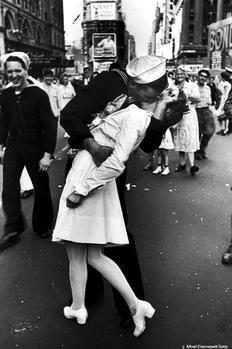
\includegraphics[width=.50\textwidth]{articles/15-cidade-em-mapas-text/enfermeira-marinheiro.jpeg}%
        \caption*{Fonte: \textcite[p.~90]{Berman2009Seculo}. Autor: Alfred Eisenstaedt.}%
        \label{fig:enfermeira-marinheiro}%
    \end{figure}%

    Há imagens que ficam, realmente. Barthes entende que cada imagem tem diferentes significados, dependendo do momento de produção e de interpretação, cuja ligação é o referente que se cria/possui \cite{Barthes2015Camera}. O produzir/ler a fotografia é, portanto, cultural. Tal abordagem se revela fecunda quando inventariamos aquilo que nos marcou, entre tudo que vimos. 

    Há imagens que ficam, ratificamos. Como as da cidade de São Paulo nas primeiras décadas do século anterior. São fotografias que circularam em cartões postais e revistas ilustradas, construindo uma cidade em transição de província para metrópole; de Piratininga para São Paulo. Imagens que ainda se revelam poderosas. Vendo-as, o sentimento de nostalgia de um tempo pretérito, com ares bucólicos, mistura-se ao novo sentir de uma época que principia sua aceleração. A fotografia de Guilherme Gaensly (figura \ref{fig:estacao-luz}), uma panorâmica da Estação da Luz, com seus trilhos que remetem ao progresso econômico e tecnológico, coexistem com as carroças responsáveis pelo abastecimento da cidade. O bonde elétrico, que passa em frente à estação, é, também, alusão à metrópole que se faz. Essa imagem, que cruzou estradas e oceanos em cartões postais, discursa sobre o feito e sobre o se fazer; discursa, portanto, sobre oportunidades. A fotografia que hoje decora, junto com outras, estabelecimentos paulistanos é, ainda, o se constituir possível, na São Paulo, onde garoa e trabalho configuram definições corriqueiras e historicamente construídas.

    \begin{figure}[ht]%
        \centering%
        \caption{Estação da Luz, São Paulo, 1905--6}%
        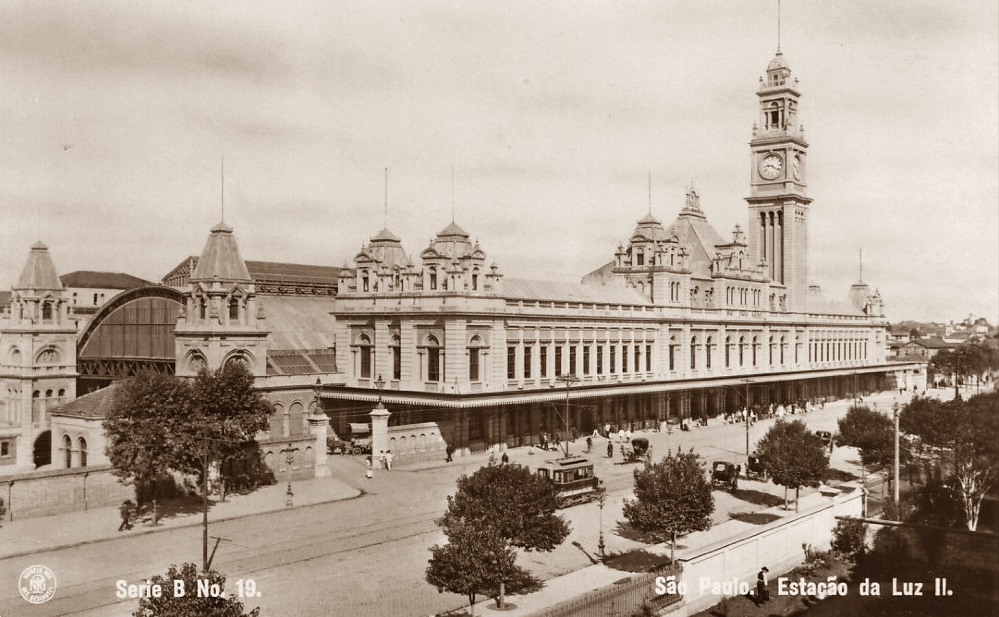
\includegraphics[width=.85\textwidth]{articles/15-cidade-em-mapas-text/estacao-luz.jpeg}%
        \caption*{Fonte: \textcite[p.~80--81]{KossoyFernandesJuniorAndSegawa2011Guilherme}. Autor: Guilherme Gaensly.}%
        \label{fig:estacao-luz}%
    \end{figure}%

    Analisando outras fotos e postais de Gaensly, novo aspecto desperta atenção. Tamanha é a força do que foi captado pelas objetivas, que a memória que possuímos, desse tempo que não vivemos, por isso, memória construída por diversas impressões, é a de um tempo em preto e branco, um tempo difícil de imaginar com suas cores cotidianas. É, também, um tempo mudo. Rápido, mas silencioso, como em ``São Paulo, a Symphonia da metrópole'' \citeyear{KemenyAndRex1929Sao}: o dia citadino é veloz, num correr que não se ouve, mas se percebe. O que faz essas imagens viverem em dinâmica conflituosa, emitirem sons e exalarem odores, é a literatura:

    \begin{quotation}
        \settowidth{\versewidth}{Bondes desabalando frenesis de velocidades}
        \noindent\begin{verse}[\versewidth]
            A multidão arrastando-se na cidade\\
            O tripudiar de um pique de cavalaria\\
            Bondes desabalando frenesis de velocidades\\
            Um milhão de máquinas de escrever batendo frenética simultaneamente todas as suas teclas (\dots)\\
            Os telefones desabaladamente as campainhas\\
            A raiva do que pede ligação pela quinta vez!\\
            Os carros de bombeiros rolando paralelepípedos \\
            Apitos vozaria e alaridos\\
            O atropelo dos automóveis depois de um grande match de foot-ball\\
            Buzinas rouquidões motores algazarras\\
            O Vento correndo sobre pneumáticos\\
            Rugindo pelo espaço\\
            Porque ele é um automóvel que buzina (\dots)
        \end{verse}

        \noindent\begin{verse}[\versewidth]
            \cite[p.~39--40]{Aranha1984Cocktails}
        \end{verse}
    \end{quotation}

    O trecho do poema ``Drogaria de éter e de sombra'', de Luis \textcite{Aranha1984Cocktails}, é construído pelos vocábulos que se fizeram presentes nas falas paulistanas, advindos com o desenvolvimento urbano. Por ele, somos imersos no clima de uma cidade repleta de choques e atropelos --- que desnorteiam, mas também encantam quem por ela transita, como o poeta:

    \begin{quotation}
        \settowidth{\versewidth}{Bebo com lábios que sussurram}
        \noindent\begin{verse}[\versewidth]
            De tarde\\
            A luz andava\\
            No vale verde do Anhangabaú\dots\\
            Oh! O seu canto louro e triunfal\\
            Seu exaltado canto de agonia! (\dots)\\
            Amo a tarde de carnes incendiadas\\
            Que me penetra e que lateja em mim!\\
            Bebo com lábios que sussurram\\
            Este vinho de luz que jorra pelo espaço\\
            Até sentir a embriagues da luz\dots\\
            Estes rios de sons que golfam do ocaso\\
            Incendiados de clarins\\
            Penetram na minha alma ressequida\\
            Com tanto ímpeto e com tal ardor\\
            Que sinto em mim resplandecer a vida! \dots\\
            Ardo na exaltação que os passos me conduz\\
            E não sinto meu peso sobre a terra\\
            Porque meu corpo é um jato de luz! \dots
        \end{verse}

        \noindent\begin{verse}[\versewidth]
            \cite[p.~40--41]{Aranha1984Cocktails}
        \end{verse}
    \end{quotation}

    O diálogo entre tipos de linguagens e representações permite a construção, não total, mas abrangente, de um painel desse período. Muitos intelectuais trouxeram para seu fazer jornalístico e literário a sonoplastia, a paleta de cores e o movimento da urbe paulistana. Muitos representaram a ambiguidade de sentimentos diante da metrópole que se edificava: um desejo por sensações contraditórias, por uma adrenalina que, paradoxalmente, confortava.  Menotti del Picchia, Mario e Oswald de Andrade, também deixaram impressas visões conflituosas diante da vertigem urbana. No entanto, foi António de Alcântara Machado, ``o prosador do modernismo paulista'' \cite[p.~400]{Bosi2006Historia}, quem melhor permitiu o sentir da cidade por meio do texto, não apenas pelo enredo, mas igualmente pela forma, que incorpora recursos diversos na organização da narrativa. Em António, o espaço em branco fala, ou melhor, convida o leitor a dizer, a participar da narrativa, a realizar a transição espaço-temporal. Em outras palavras: além da trama desenrolada na urbe --- de cartografia ampliada ---, além dos vocábulos citadinos, a disposição textual alude ao movimento, cheiro, sons. Olhar um postal de Gaensly, com o saboroso poema de Luis Aranha, faz a imagem reviver; olhar um postal de Gaensly, com a prosa de Alcântara Machado, permite que vivamos a imagem. Pelos seus registros, ratificamos, a cidade se tinge em cores, exala incontáveis aromas, fala seus sons. Existe:

    \begin{quotation}
        Eu me sentirei no alto, mas muito no alto. São Paulo então não abandonará seu filho. Com cheiro de gasolina, com fumaça de fábrica, com barulho de bondes, com barulho de carros, carroças e automóveis, com barulho de vozes, com cheiro de gente, com latidos, cantos, pipilos, assobios, com barulho de fonógrafo, com barulho de rádio, campainhas, buzinadas, com cheiro de feiras, com cheiro de quitandas, todos os cheiros e também barulhos da vida, São Paulo encherá o silêncio da morte. \cite[p.~148]{Machado1970Meditatio} 
    \end{quotation}

    O encadeamento, como a lógica confusa da cidade, entrega o cotidiano apressado, vivo. A construção narrativa de António de Alcântara Machado coloca-nos em simultaneidade. Pela mão do autor, estamos em inúmeros lugares ao mesmo tempo. Ler António, com atenção na prosa construída, já é adentrar na São Paulo dos anos vinte e suas sociabilidades modernas.  

    Essa técnica, deliberada, sempre esteve em seu horizonte, desde a obra de estreia nos moldes modernistas, ``Pathé-Baby'' (1926): pela linguagem, construir uma prosa pura, documental, limada dos excessos, adjetivos e longos períodos; edificar, assim, um texto ágil, de acontecimentos síncronos; em poucas páginas, um bairro inteiro.

    \section{Gaetaninho}

    Em 1927, António de Alcântara Machado publicou seu segundo livro, ``Brás, Bexiga e Barra Funda''. Bem aceito pelo crítica, recebeu elogios calorosos. Stiunirio Gama, pseudônimo de Mário Guastini, em longa crítica no Jornal do Comércio, afirma que: 

    \begin{quotation}
        (\dots) \textit{Brás, Bexiga e Barra Funda} é um livro delicioso. E o é, de fato; sem favor. Os contos que reúne em suas páginas são verdadeiras jóias literárias. Qualquer um deles, ao acaso, agradará. E mesmo que assim não fosse bastaria um, um apenas, para confirmar o indiscutível valor de Antonio de Alcântara Machado. \cite[p.~92]{Gama1984Segundas}
    \end{quotation}


    Martin Damy diz que se trata de ``um livro profundo, com aparências de coisa banal'' \cite[p.~101]{Damy1984Espirito}. João Ribeiro, pelo Jornal do Brasil, escreve que ``o livro de Alcântara Machado é um grande exemplo da literatura nova'' \cite[p.~102]{Ribeiro1982Bras}.  

    É de ``Brás, Bexiga e Barra Funda'', talvez, suas mais conhecidas produções: ``Gaetaninho'', o garoto que tem a vida abreviada pelo bonde; ``Carmela'', a costureirinha da Barão de Itapetininga, que mistura, no corpo e trejeitos, a inocência provincial com a sedução metropolitana; e ``Lisetta'', a menina que se encanta com um ursinho, enquanto transita de bonde pela cidade, numa narrativa extremante sensível em seu riso. No presente artigo, nosso escopo é um pedaço do Brás: a Rua Oriente, e seu jogo de vida e morte.   

    Sobre Gaetaninho, conto que abre ``Brás, Bexiga e Barra Funda'', Rodrigo Andrade, n'O Jornal: ``pode ser lido em dez minutos. Mas faz pensar muito tempo e não sai mais da memória da gente'' \cite[p.~95]{Andrade1982Vida}.  

    O personagem é fruto do cosmopolitismo que caracteriza São Paulo como cidade moderna. Em Alcântara Machado, o cosmopolitismo não se encontra apenas nos salões, mas também nos bairros operários. O autor chama a atenção aos múltiplos sentires que a cidade provoca, a depender da condição social. Descreve a situação do imigrante pobre diante de um meio que agrega e exclui. E seduz --- sedução de morte.  

    Gaetaninho tem o final em velório. Apesar disso, nós o lemos naquele estado que antecede o sorriso de camaradagem, diante da leveza.  Pela narrativa, o menino que joga bola experimenta a fronteira borrada entre a rua como espaço lúdico e via de passagem automotiva. O atropelamento, como desfecho, representa o lado que diluiu, por completo, o momento de transição, afirmando-se. Desde o início, a relação entre homem, máquina e espaço é explorada.  

    \begin{quotation}
        Gaetaninho ficou banzando bem no meio da rua. O Ford quase o derrubou e ele não viu o Ford. O carroceiro disse um palavrão e ele não ouviu o palavrão. \cite[p.~20]{Machado2003Contos}
    \end{quotation}

    O vocábulo Ford leva a metonímia para uma definição além de si mesma: mais do que conter o todo, pela parte, sinaliza a despersonalização do homem diante da máquina \cite{Silva2010Bras}. O quase atropelamento alerta o garoto de que o espaço de folguedos vai se fazendo utilitário. Mesmo o carroceiro, elemento humano que com ele estabelece uma relação humana, ainda que ofensiva --- mas ofensividade que serve de alerta e preservação --- também caminha para a extinção, diante metrópole que se desenvolve. A máquina se impõe e toda lógica urbana tende a favorecer sua circulação em detrimento do ser. No recorte seguinte, pela técnica narrativa cinematográfica de Alcântara, que vai de planos fechados (em Gaetaninho), para abertos (a Rua Oriente), vemos como a mecânica fria de aços e pistões é entendida como nova regente da vida: 

    \begin{quotation}
        Ali na Rua Oriente a ralé quando muito andava de bonde. De automóvel ou carro só mesmo em dia de enterro. De enterro ou casamento. \cite[p.~20]{Machado2003Contos}
    \end{quotation}

    A máquina pontua o término (enterro); a máquina pontua a nova vida (casamento). As relações tendem à mecanização. O progresso reconfigura as interações sociais. É em tom radiofônico que a morte do garoto é narrada:

    \begin{quotation}
        O jogo na calçada parecia de vida e de morte (\dots)  

        Gaetaninho voltou para o seu posto de guardião. Tão cheio de responsabilidades. 
    
        O Nino veio correndo com a bolinha de meia. Chegou bem perto. Com o tronco arqueado, as pernas dobradas, os brações estendidos, as mãos abertas, Gaetaninho ficou pronto para a defesa.  
    
        --- Passa para o Beppino! 
    
        Beppino deu dois passos e meteu o pé na bola. Com todo muque. Ela cobriu o guardião sardento e foi parar no meio da rua.  
    
        --- Vá dar tiro no inferno! 
    
        --- Cala a boca, palestrino! 
    
        --- Traga a bola! 
    
        Gaetaninho saiu correndo. Antes de alcançar a bola um bonde o pegou. Pegou e matou.  
    
        No bonde vinha o pai de Gaetaninho. \cite[p.~21--22]{Machado2003Contos}
    \end{quotation}


    E é em tom de nota de jornal que a morte é anunciada, pois é morte de garoto pobre. Curta. Seca. Estatística. Gaetaninho perde no jogo da vida. O bonde que trazia seu pai possui amarga ironia, na qual se sinaliza o divórcio das relações pessoais, agora mediadas pelo aço: filho-bonde-pai. \cite{Silva2010Bras}

    \section{Considerações finais}

    Como reforçamos ao longo do artigo, a cidade possui inúmeras portas de entrada. Nossa intenção foi a de explorar as possibilidades abertas pela História Cultural, buscando, no entrecruzamento de fontes, extrair as representações citadinas.  

    A ``Garota do Times'', que Berman nos traz, funciona como síntese: a linguagem gráfica é composta pelo elemento concreto da Times Tower e pelo cartum, num conjunto que representa um espaço acolhedor, convidativo: queremos, também, estar. Trata-se de uma produção de 1903, quando a Square era ainda conhecida como Longrace Square. Estamos, portanto, no início do século XX, e a experiência da modernidade é sedutora como a garota; e vertiginosa como o arranha-céu que lhe serve de suporte. Ao longo dos anos, Berman segue sua procura e encontra, nas representações da Times, a dinâmica que envolve local, vivências, sociabilidades, imagens --- e de volta, num movimento dialético entre modernização e modernismo, que para ele é a essência da modernidade.  

    De nossa parte, perscrutamos, em outro contexto, a vida --- e morte --- que existe nos mapas. Pela Rua Oriente, o sonho e o jogo de Gaetaninho a revelar temporalidades distintas, no avanço da metrópole sobre a província. Avanço que não se confirma apenas pela expansão, demografia, gráficos e tabelas. Mas ratifica-se pelas possibilidades que oferece e nega, pelos laços comunitários e lúdicos que rompe. E os habitantes, ainda que vitimados, posicionam-se, reivindicam a urbe para si. Ressignificam os mapas.

    \printbibliography[heading=subbibliography,notcategory=fullcited]

    \hfill Recebido em 15 abr. 2021.

    \hfill Aprovado em 19 abr. 2021.

    \cleardoublepage

    \begin{vplace}
        \section*{Anexos: plantas da cidade de São Paulo}
        \addcontentsline{toc}{section}{Anexos: \textit{plantas da cidade de São Paulo}}
    \end{vplace}

    \clearpage

    \rannex{annex:sp1916}
    \begin{vplace}
        \centering
        \begin{tikzpicture}
            \node[] (mapa1916) at (0, 0)
                {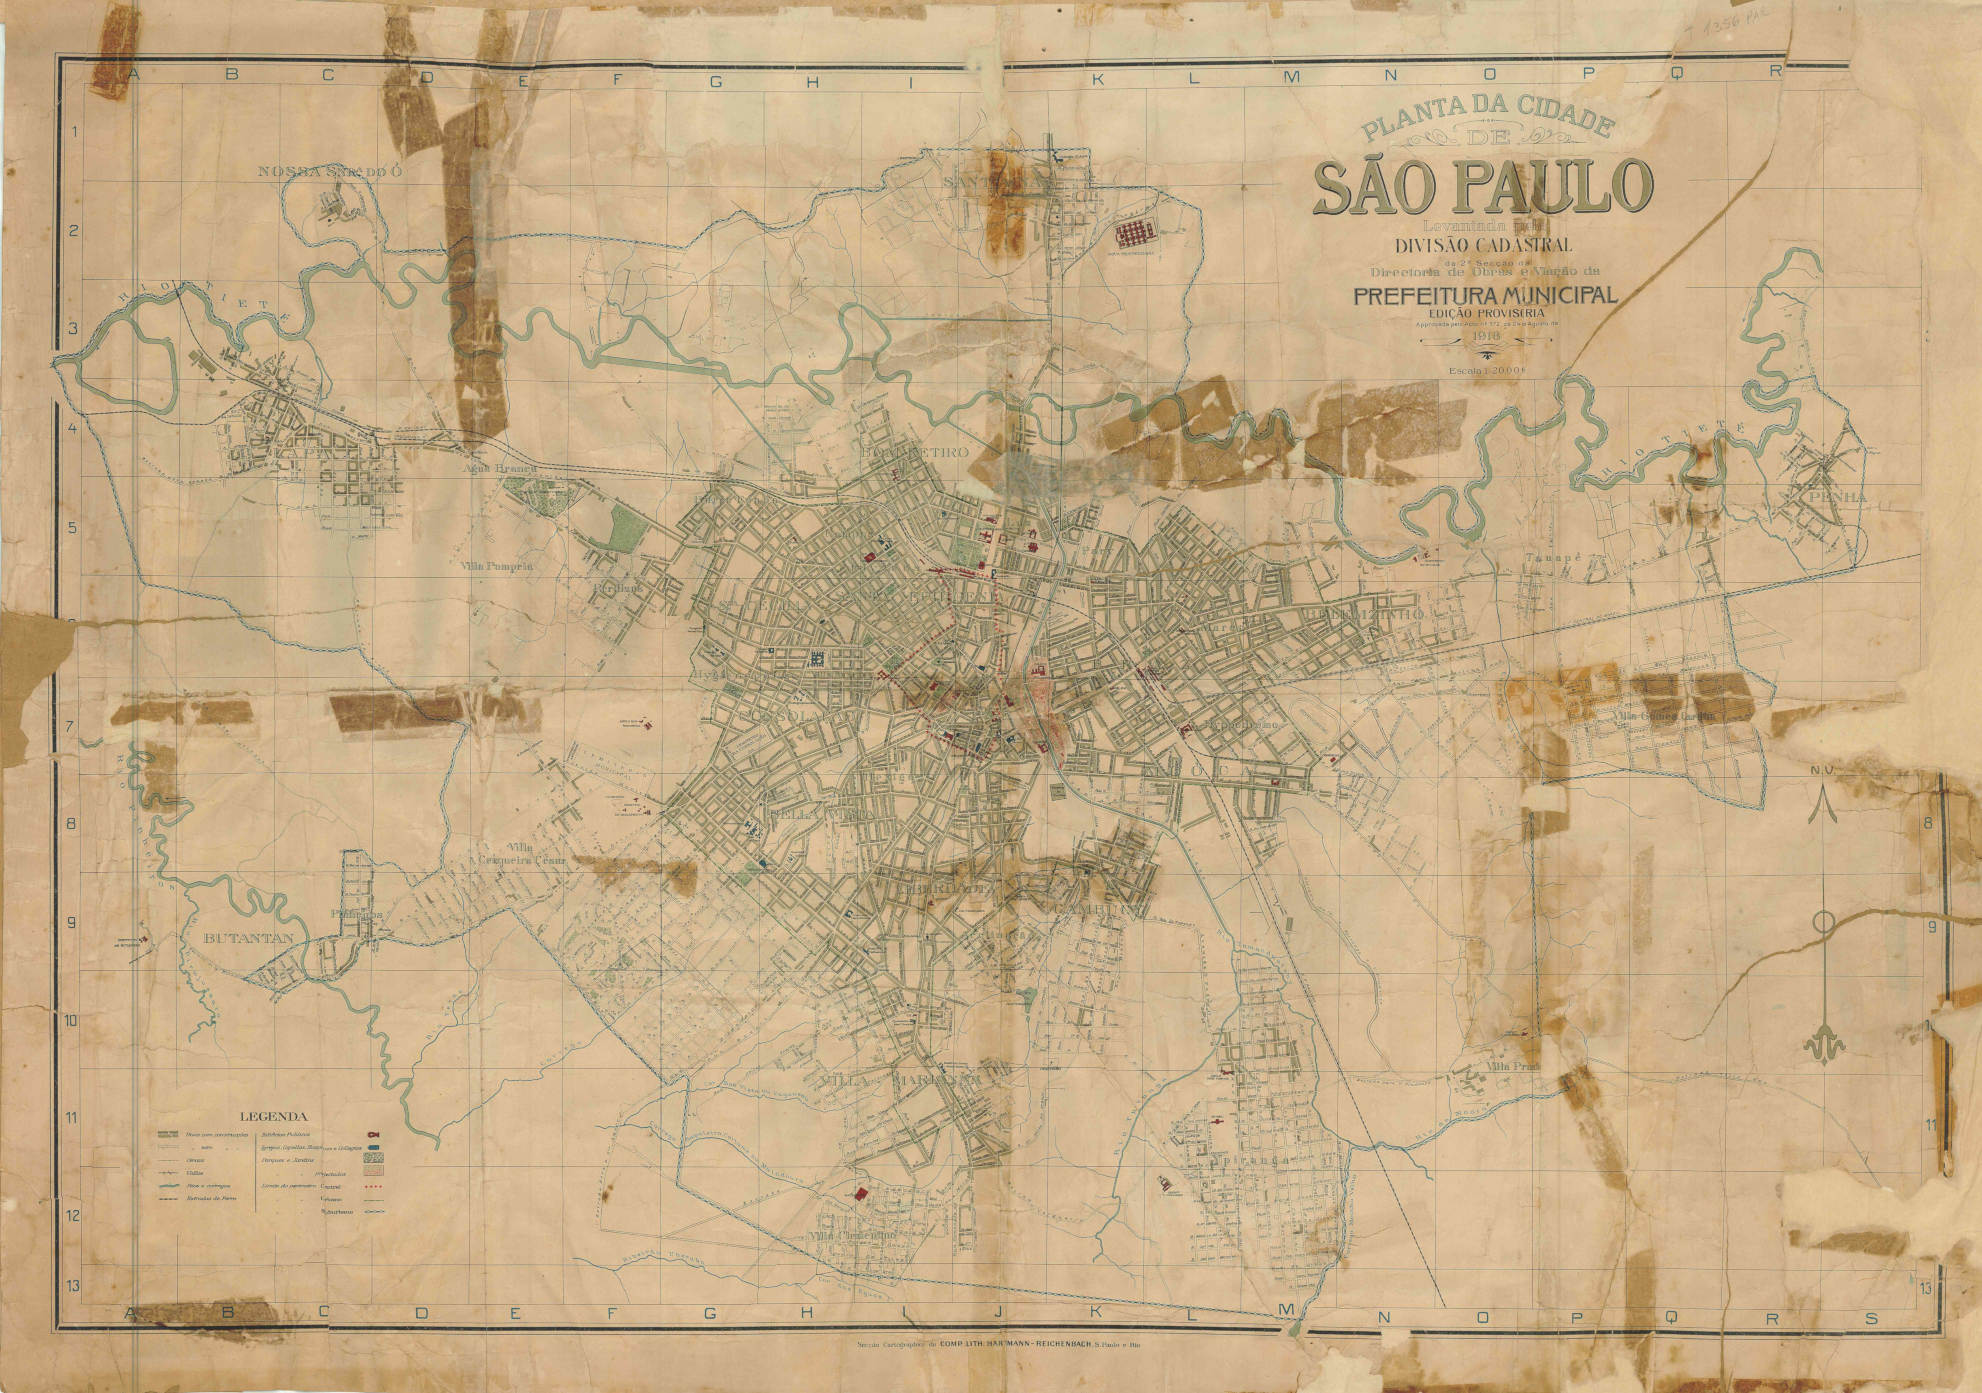
\includegraphics[width=\textwidth]{articles/15-cidade-em-mapas-text/planta-sp-1916.jpg}};
            \node[anchor=north west, text width=\textwidth] (caption) at ([yshift=-5mm]mapa1916.south west)
                {\small \textsf{Anexo \ref{annex:sp1916} -- Planta da Cidade de São Paulo. 1916. Disponível em \url{http://smul.prefeitura.sp.gov.br/historico_demografico/img/mapas/1916.jpg}. Acesso em 15 abr. 2021.}};
        \end{tikzpicture}
    \end{vplace}

    \clearpage

    \rannex{annex:sp1924}
    \begin{vplace}
        \centering
        \begin{tikzpicture}
            \node[] (mapa1924) at (0, 0)
                {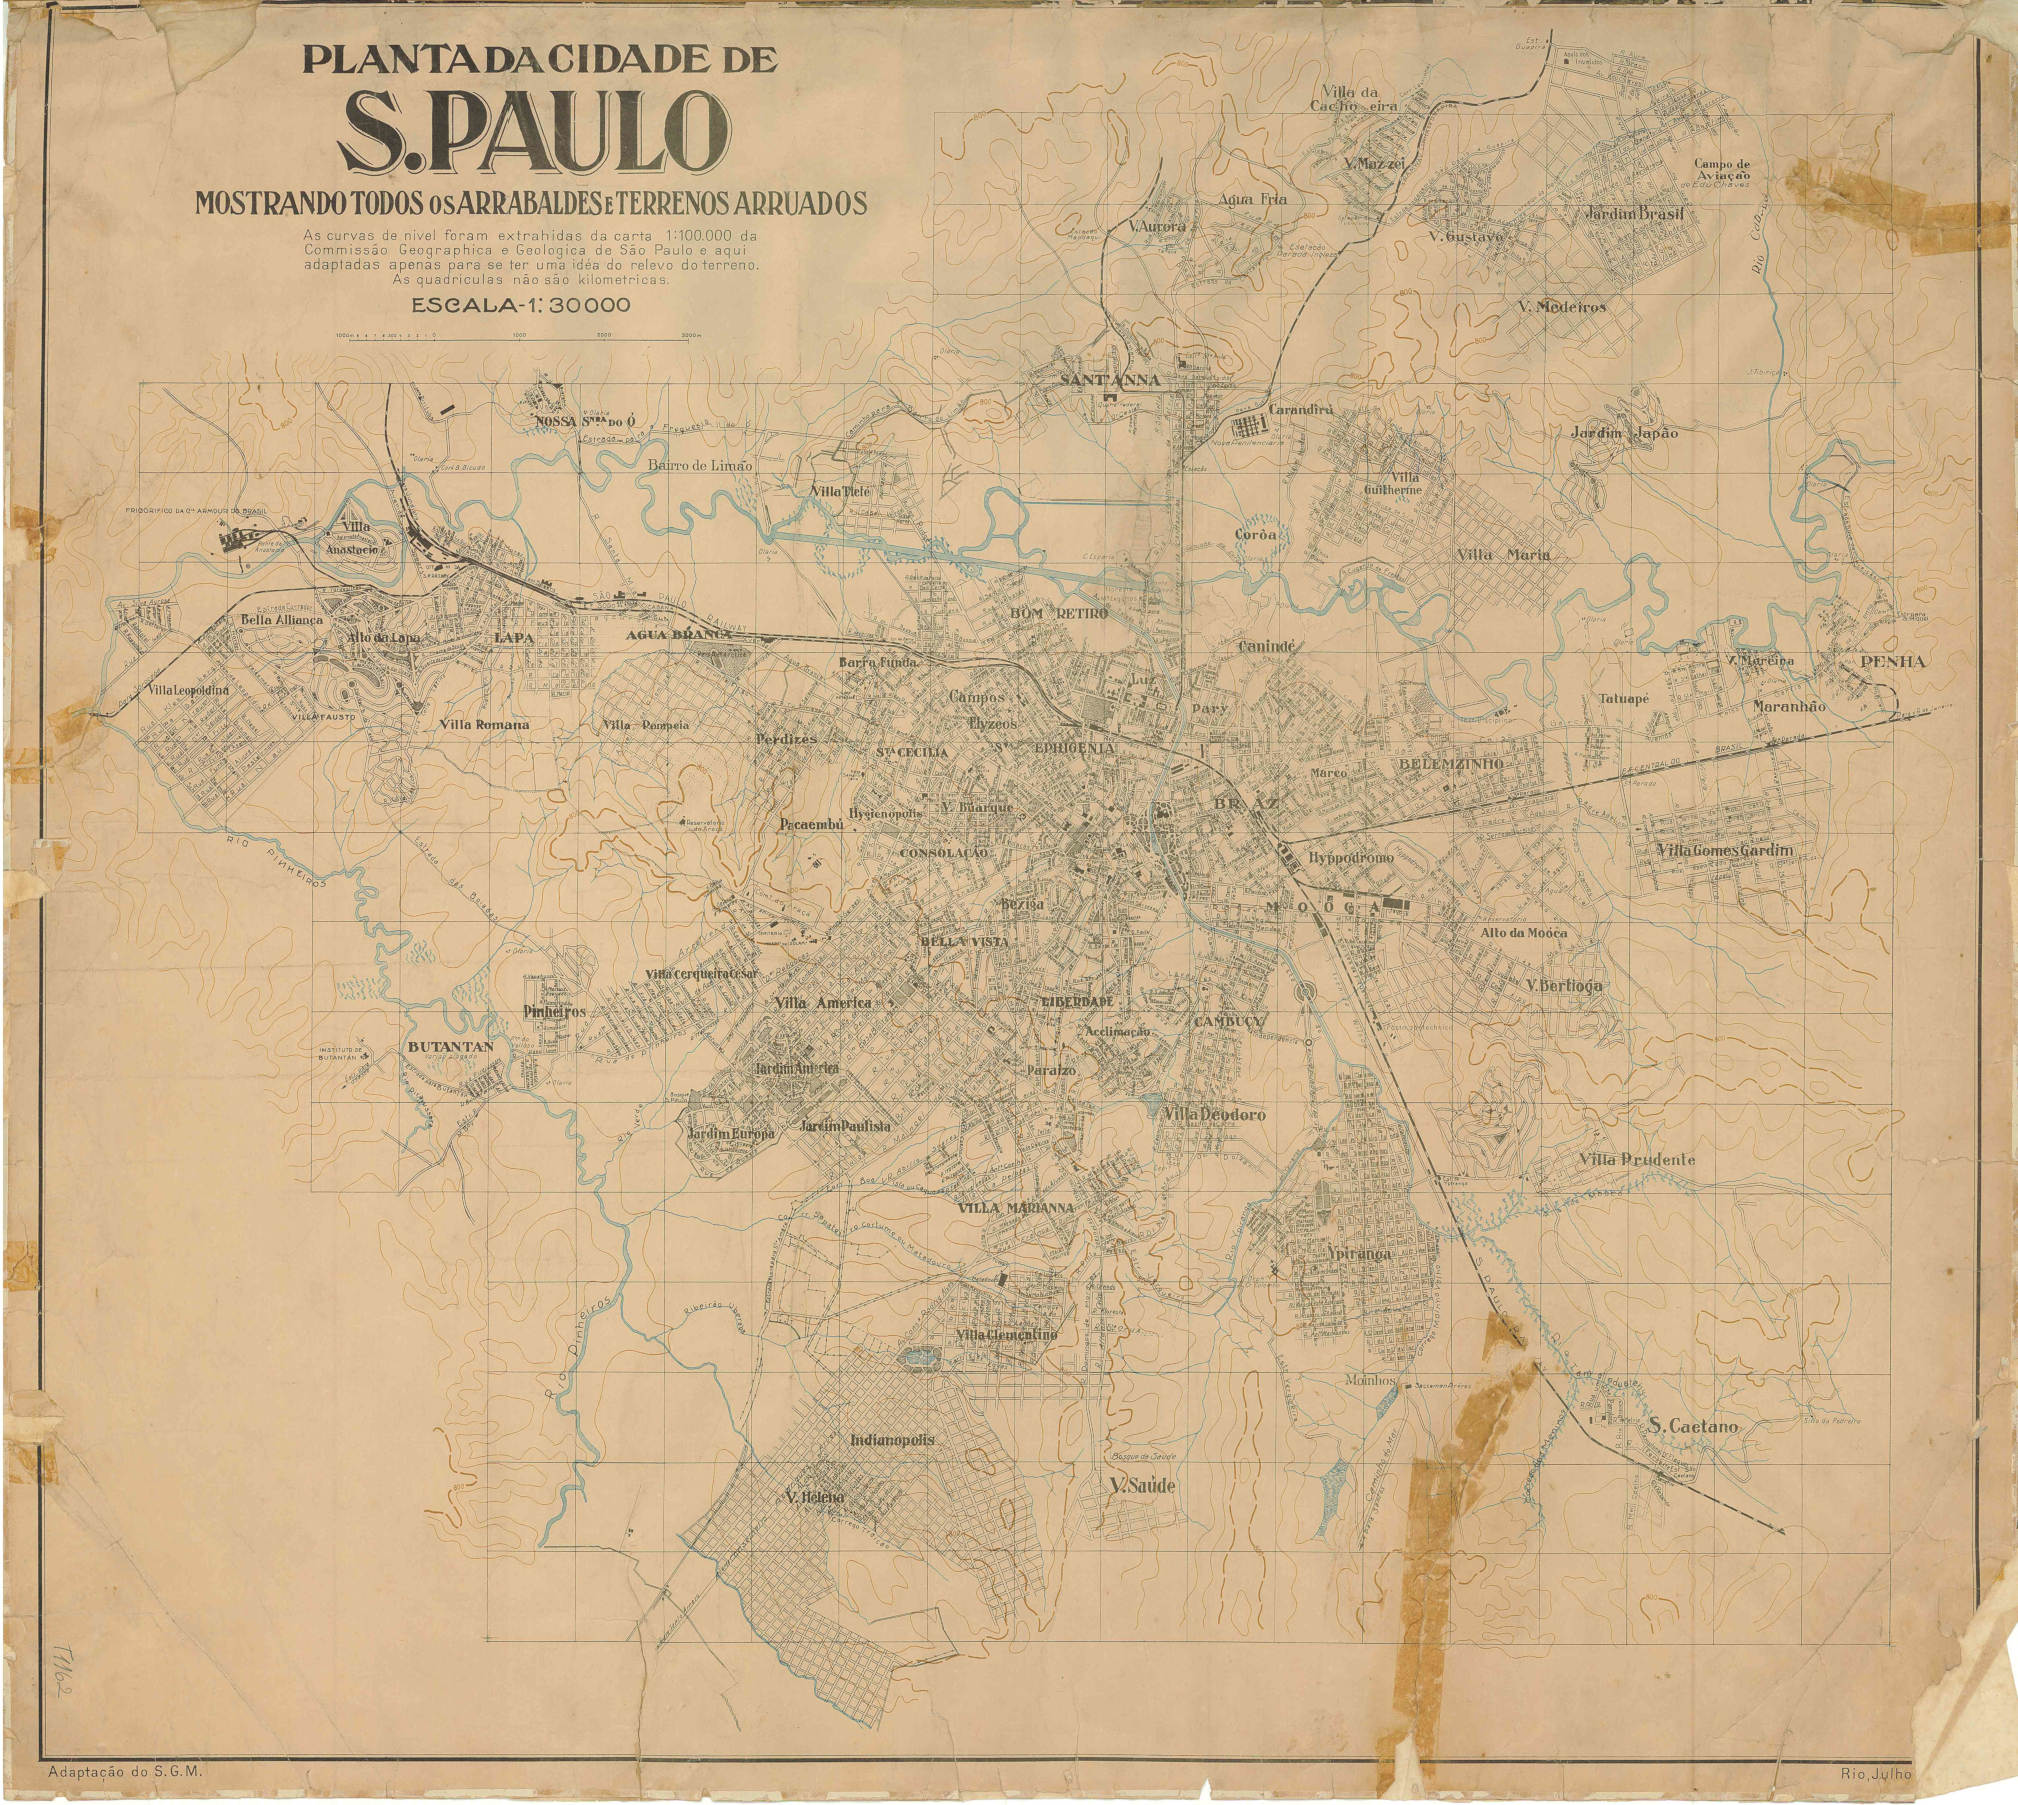
\includegraphics[width=\textwidth]{articles/15-cidade-em-mapas-text/planta-sp-1924.jpg}};
            \node[anchor=north west, text width=\textwidth] (caption) at ([yshift=-5mm]mapa1924.south west)
                {\small \textsf{Anexo \ref{annex:sp1924} -- Planta da Cidade de São Paulo. 1924. Disponível em \url{http://smul.prefeitura.sp.gov.br/historico_demografico/img/mapas/1924.jpg}. Acesso em 15 abr. 2021.}};
        \end{tikzpicture}
    \end{vplace}

    \clearpage

    \label{chap:mapadacidadeend}

\end{refsection}
